\chapter{双模式检查点生成技术}
\label{chap:thynvm}

新兴的按字节编址的(byte-addressable)非易失性内存介质,诸如STT-RAM~\cite{4443191,6557176}、PCM~\cite{Raoux:2008:PRA, 10.1109/MM.2010.24}和ReRAM~\cite{5607274}等,预示着持久化内存系统的兴起。持久化内存可能发展成为内存和存储栈中一个新的中间层。持久化内存系统融合了传统内存系统(快速的load/store指令接口)和存储系统(数据持久化)的优良特性,模糊了两者之间的界限。它给应用带来的一个重要的益处是,可以通过load/store指令高效地直接地访问内存中的持久化数据,而不需要与存储设备进行页交换(page swapping)、在(反)序列化时更改数据格式以及触发臃肿的系统调用~\cite{meza2013case}。

持久化内存相对于传统的易失性内存系统引入了一个关键的要求,系统故障时的一致性保证~\cite{Lamb:1991:ODS,Copeland:1989:CSR,Shapiro:1999:EFC:319151.319163}。这要求持久化内存系统,在掉电或系统失效等故障出现时,依然能够保证数据的一致性不受部分的或是乱序的NVM写的影响。我们以原子性地更新保存在NVM上的数据结构A和B为例,总会有对A或B的一个更改会先于另一个写入NVM。如果系统在一个更改完成之后出现故障或掉电,两个数据结构可能处于不一致的中间状态,只包含部分更改。对于传统易失性内存,这不是一个问题,因为程序恢复后内存中的数据都会丢失。但对于持久化内存,这些不一致的数据会一直保留。所以,持久化内存系统需要保证保存到NVM的数据可以在系统重启后恢复到一个一致的状态,即维持数据的一致性。维持数据的一致性原本仅是对磁盘或闪存等存储系统的要求,但将数据持久化引入内存后,它即成为内存系统同样面临的一个挑战。

大多数之前的持久化内存设计依赖于程序员的人工努力来保证系统故障时的数据一致性\cite{
  Volos:2011:MLP:1950365.1950379, Coburn:2011:NMP:1950365.1950380,
  Venkataraman:2011:CDD:1960475.1960480, Intel:PMEM,
  Zhao:2013:KCP:2540708.2540744, Pelley:2014:MP}。应用的开发人员需要显式地使用特定的编程模型和软件接口来访问和操作内存中的持久化数据,以保护数据一致性不受部分写或是乱序写的影响。这种方式似乎给程序员提供了对数据持久化的完全控制,但要求程序员使用新接口管理持久化内存会带来多方面不良影响。首先,程序员必须用新的编程接口API来实现程序或者深度更改遗留代码,通常要显式地声明和划分持久的和临时的数据结构。其次,已经部署在各种系统中的使用遗留代码的应用无法利用持久性内存系统。第三,大多数之前的持久化内存设计需要使用事务性内存控制版本和对NVM写的顺序,而事务性内存的扩展性依然面临挑战\cite{Cascaval:2008:STM:1454456.1454466, Pankratius:2011:STM:1989493.1989500, Dice:2009:EEC:1508244.1508263}。第四,持久性内存应用的实现依赖特定的软件接口和运行时系统\cite{Volos:2011:MLP:1950365.1950379, Coburn:2011:NMP:1950365.1950380, Venkataraman:2011:CDD:1960475.1960480, Intel:PMEM, SNIA:2013:NPM},会带来跨系统的兼容性和移植性问题

本章工作的\textbf{目标}是为持久性内存系统设计高效的\emph{对软件透明的}故障时数据一致性保证机制。我们希望这样的设计可以使更多持久性内存的用例成为可能(如用于不修改的遗留程序或者非事务性的程序),并允许更多的程序员使用持久性内存系统而不必更改应用来保证数据一致性。

为此,我们提出了ThyNVM,一种新的支持对软件透明的故障时数据一致性的基于DRAM和NVM混合架构的持久化内存系统。它允许基于事务的和非事务性的程序直接在持久化内存硬件上运行,而且获得完整的故障时数据一致性支持。ThyNVM通过定期地在硬件辅助下生成检查点来保证系统在故障时可以恢复到一个一致的内存状态。然而,一般的检查点生成技术需要在将数据持久化到NVM的过程中令整个系统停顿。减少由于使用检查点生成技术导致的程序停顿是此类系统面临的关键挑战。

ThyNVM采用两个方法减少检查点生成的开销。第一,它将检查点生成过程和程序执行过程重合。第二,为了高效地支持这种重合,它动态地决定数据生成检查点的粒度。该决定依据我们新的观察,即在应用停滞时间和元数据存储开销之间存在一个权衡。在较小的粒度上生成检查点,带来的停滞时间比较短,而对应元数据占用的空间却会非常大;在较大的粒度上生成检查点,可以降低元数据占用的空间,但是会导致较长的停滞时间。因此,单一的检查点生成技术(或者基于小粒度或者基于大粒度)难以达到最优的效果。为了解决这一问题,我们提出了\emph{双模式检查点生成机制},它可以同步地为分散的(低空间局部性)和集中的(高空间局部性)内存写分别基于CPU缓存块粒度和操作系统页粒度生成检查点。与使用日志\cite{Volos:2011:MLP:1950365.1950379, Coburn:2011:NMP:1950365.1950380}或写时拷贝(copy-on-write,COW)\cite{Condit:2009:BIT:1629575.1629589, Venkataraman:2011:CDD:1960475.1960480}的持久化内存设计相比,ThyNVM显著减小了存储的损耗并增加了内存带宽的利用率。

综上,本章工作做出了如下几点贡献:(1)我们提出了一种新的持久化内存设计,支持\emph{对软件透明}的故障时数据一致性保障。我们的设计允许基于事务的和无修改的遗留应用通过load/store指令接口使用持久化内存。(2)对于生成检查点的粒度,我们定位了\emph{应用停滞时间和元数据空间开销之间的权衡关系}。在任意一个粒度上生成内存数据的检查点都不是最优的。(3)我们设计了一个新的\emph{双模式检查点生成}技术。我们发现,低空间局部性的更改最好以细粒度生成检查点,而高空间局部性的更改最好以粗粒度生成检查点。我们的设计比页粒度的检查点生成机制减少了86.2\%的停滞时间,而仅用块粒度的检查点生成机制所需硬件空间的26\%(位于内存控制器)。(4)我们在内存模拟器上使用我们经过形式化证明的一致性协议实现了双模式检查点生成机制。它可以在保证数据一致性的同时,通过将程序执行和检查点生成过程重合获得高性能。我们的解决方案可以达到不提供一致性支持的全DRAM系统性能的95.1\%。

\section{软件透明的一致性保证机制}

ThyNVM包含了两个设计选择:(1)对故障时数据一致性的支持是软件透明的,而不是依赖软件技术;(2)故障时数据一致性机制是基于检查点生成技术,而不是日志或写时拷贝。本节讨论采用这些技术选择的原因。

\subsection{软件一致性保障技术的缺陷}

\begin{figure}[!h]
\centering \includegraphics[width=0.85\linewidth]{motivation-code}
  \caption{实例代码:向持久化的哈希表中插入一个项。分别采用(a)传统的软件接口或(b)软件透明的ThyNVM。}
\label{fig:motivation-code}
\end{figure}

之前大多数持久化内存设计~\cite{Condit:2009:BIT:1629575.1629589, Volos:2011:MLP:1950365.1950379, Coburn:2011:NMP:1950365.1950380, Zhao:2013:KCP:2540708.2540744, Venkataraman:2011:CDD:1960475.1960480}要求应用开发者显式地定义持久性数据并使用特定库来访问数据——故障时数据一致性保障机制与软件的语义紧耦合。我们通过图\ref{fig:motivation-code}中的实例代码来展示这种持久化内存设计的不足。该图比较了一个更新持久性哈希表项的软件方法的两种实现(代码改编自STAMP~\cite{Cao:2008:STA})。图\ref{fig:motivation-code}(a)展示了使用类似于现有设计~\cite{Condit:2009:BIT:1629575.1629589, Volos:2011:MLP:1950365.1950379}的软件事务的实现;而图\ref{fig:motivation-code}(b)中的实例代码采用了ThyNVM的对软件透明的故障时数据一致性保证机制。我们可以看到,在支持数据一致性时涉及软件支持,会有多方面的不足。

首先,手工划分临时性和持久性数据很麻烦而且容易出错。图\ref{fig:motivation-code}(a)展示了许多无法避免的标记。程序员需要对软件行为有深入的了解,并且小心地确定哪些数据结构需要持久化以及如何操控这些数据。例如,图\ref{fig:motivation-code}(a)的第3行从哈希表中读出一个链表。该行仅当这个哈希表实现固定数目的链表时才是正确的。否则,另一个并发线程可能正在重置这些链表而导致错误。为了防止这个问题出现,程序员需要使用事务,来保护对链表的访问(程序第3行)不受并发线程的影响。

其次,在一个统一的地址空间内,临时性和持久性数据之间的引用需要小心的管理。然而,对该问题的基于软件的解决方案并非最佳。例如,为了处理NV-to-V指针(非易失性指针指向易失性数据,图\ref{fig:motivation-code}(a)的第8行),NV-heaps~\cite{Coburn:2011:NMP:1950365.1950380}会简单地抛出一个运行时错误以禁用此类指针。

第三,应用需要使用事务,通常是通过事务性内存接口(例如被Mnemosyne~\cite{Volos:2011:MLP:1950365.1950379}使用的TinySTM~\cite{Felber:2008:DPT}),来更新持久化数据,如图\ref{fig:motivation-code}(a)所示。然而,不论基于硬件的还是基于软件的事务性内存,都存在多方面的可扩展性问题~\cite{Cascaval:2008:STM:1454456.1454466, Pankratius:2011:STM:1989493.1989500, Dice:2009:EEC:1508244.1508263}。此外,开发人员必须使用新的API来实现或者重写各种代码库和程序,需要不可忽略的人工投入。不熟悉这些新API的程序员需要一个痛苦的学习过程。

最后,应用需要构建在特定的库之上,例如libmnemosyne~\cite{Volos:2011:MLP:1950365.1950379}和
NV-heaps~\cite{Coburn:2011:NMP:1950365.1950380}。这会很大程度上降低持久化内存应用的移植性——在一个库上实现的应用,如果想采用其他的库,需要重新实现。编译器插装确实可以在一定程度上减轻程序员实现和移植代码的负担。然而,编译器会无差别地插装所有(或大部分)内存的读和写操作,带来可见的性能损耗。我们在GCC libitm~\cite{libitm}上实验了STAMP事务性标准测试~\cite{Cao:2008:STA},结果插装本身最多可带来高达8\%的性能损失。

我们采用了允许软件程序直接访问持久化内存而无需特别的支持故障时数据一致性的接口的使用模型。如图\ref{fig:motivation-code}(b)所示,我们可以不更改代码而实现数据结构的持久化。

\subsection{日志及写时拷贝技术的缺陷}

现有基于软件的持久化内存设计多采用日志~\cite{Volos:2011:MLP:1950365.1950379, Coburn:2011:NMP:1950365.1950380}或者写时拷贝技术~\cite{Condit:2009:BIT:1629575.1629589,
Venkataraman:2011:CDD:1960475.1960480}维持数据一致性。基于日志的系统在日志中维护原始数据的额外副本,用以保存新的数据更新(重做日志)或者旧的数据值(撤销日志)。基于写时拷贝的系统在数据更新时会创建一个新的副本用于更新。然而,两种技术为支持数据一致性保障会引入较大的性能损耗。

日志可能消耗比原始数据大很多的NVM空间,因为每个日志项都是一个既包含数据又包含元数据(例如数据所在的地址)的元组,而且通常每次写操作都需要记录~\cite{Volos:2011:MLP:1950365.1950379,
Coburn:2011:NMP:1950365.1950380}\footnote{某些对于日志的改进或变形~\cite{1003568}使用一个索引结构来合并更新。该设计即与我们双模式之一类似。}。此外,日志重放增加了故障后系统恢复时间,会抵消使用NVM而不是顺序访问的块设备带来的快速数据恢复的好处。

写时数据拷贝有两个缺点。首先,拷贝操作代价较大,会引发较长的停滞时间。其次,它不可避免地会复制未更改的数据,消耗额外的NVM带宽。这个缺陷在更新的地址很分散时尤为突出。

相比之下,生成检查点是一种更加灵活的方法,它定期地将易失性的数据及元数据写入NVM形成一致的内存数据的快照。我们采用检查点生成技术来克服日志和写时拷贝的弊端,但同时,降低检查点生成的开销尤为重要。为此,本章设计了新的检查点生成机制。


\section{双模式检查点生成技术}

\subsection{粒度的权衡}\label{subsec:granularity-tradeoff}

检查点生成主要是获得数据工作副本的快照(工作副本即正在被活跃地更新的数据副本),并将其持久化到NVM中(即为检查点)。检查点生成主要有两个问题:(1)生成数据工作副本检查点的延迟;(2)为追踪数据的工作副本和检查点的位置而储存的元数据的开销。理想情况下,我们希望将两者都最小化。然而,它们之间存在复杂的权衡关系。在设计高效的检查点生成机制时,我们需要考虑这些权衡关系。

首先,元数据的开销决定于我们追踪数据工作副本和检查点的粒度。我们将该粒度称为检查点粒度。通过使用较大的检查点粒度(例如操作系统页粒度),我们只需要小量的元数据即可追踪大量数据的位置。\footnote{我们可以与CPU缓存的标签(tag)类比:小的缓存块(细粒度)造成较大标签开销,而大的缓存块(粗粒度)需要较小的标签开销。}

第二,检查点生成延迟会受到数据工作副本的位置的影响。在一个混合内存系统中,工作副本可以保存在DRAM或者NVM中。我们分析了这两种选择.(1){\em DRAM}:因为DRAM写入比NVM更快,将工作副本“缓存”在DRAM中可以提升应用的写操作的性能。然而,如果我们把工作副本缓存于DRAM中,该副本需要在生成检查点的过程中被写回到NVM中,导致较长的检查点生成延迟。(2){\em NVM}:我们可以通过将工作副本保存在NVM中并在收到内存写请求时直接在NVM原地更新数据的方式来显著减小检查点生成的延迟。因为工作副本已经在NVM中持久化,检查点生成变得非常快捷:我们只需要在生成检查点的过程中将元数据持久化即可。然而,这种将工作副本保存在NVM中并做原地更新的方式,要求我们在收到应用的写操作时将工作副本\emph{重映射}到一个新的与检查点数据不同的NVM地址上。这样,应用可以在这个新的数据副本上操作而不会破坏检查点。而重映射操作的速度取决于追踪数据的粒度(即检查点粒度):细粒度可以实现较快的重映射,使得应用可以快速更新数据;而粗粒度会导致缓慢的重映射(因为要求拷贝大量数据,如整个页),进而导致写操作的延迟,使得应用长时间停顿。

综上,表\ref{tab:tradeoff}总结了检查点粒度和工作副本位置对检查点生成延迟和元数据开销的影响。

\begin{table}[!h]
  \centering
  \caption{选择不同的检查点粒度和工作副本位置构成的四种组合,以及不同组合的优势和劣势。粗体部分是决定一个组合高效或低效的主要因素。}
  \includegraphics[width=0.75\linewidth]{tradeoff}
  \label{tab:tradeoff}
\end{table}

选择小检查点粒度和在DRAM中保存工作副本(\ding{202})被认为低效的原因是,该组合会带来较大的元数据开销(相对于大检查点粒度\ding{203}),而且造成较大的检查点生成延迟(相对于在NVM保存工作副本\ding{204})。

我们认为大检查点粒度和在NVM中保存工作副本(\ding{205})构成的组合也是低效的,因为它会造成过高的重映射操作的延迟。该延迟会实时地体现在对NVM的写操作中,处于应用执行的\emph{关键路径}上。例如,如果我们在页粒度上跟踪数据,为了重映射一个写入NVM的缓存块粒度的更改,我们需要一并拷贝目标页中其他所有没有更改的缓存块到新的副本中,而且只有在这些完成后,应用才可以在该页继续进行写操作。这个重映射的开销在处理应用store指令的关键路径上。

基于对这些复杂的权衡关系的观察,我们的结论是,没有单一的检查点粒度或工作副本位置的选择可以很好地满足所有的需求。在ThyNVM的检查点生成模式中,我们设计了一个多粒度的检查点生成机制来实现多个检查点粒度和不同的工作副本位置所带来的最优特性。特别地,我们利用表\ref{tab:tradeoff}中两个具有互补权衡的\emph{部分高效}的组合:(1)在小粒度上生成检查点,将工作数据保存在NVM中并执行NVM写的重映射(\ding{204})。该组合对应于我们{\em 块重映射}模式(第\ref{subsec:block-remap}节)。(2)在大粒度上生成检查点,将工作数据保存在DRAM并回写到NVM中(\ding{203})。该组合对应于我们的\emph{页回写}模式(第\ref{subsec:page-writeback}节)。我们设计了两种模式间精巧的合作机制以实现两者的优势(第\ref{subsec:coordination}节),即同时获得较小的元数据开销和较短的检查点生成延迟。

\subsection{系统定义}
\label{subsec:thynvm-sys-def}

\begin{figure}[!h]
\centering
\includegraphics[width=0.8\linewidth]{thynvm-arch}
\caption{ThyNVM的总体架构图。}
\label{fig:thynvm-arch}
\end{figure}

\textbf{系统架构}:ThyNVM采用DRAM和NVM的混合架构,基于硬件实现,提供对软件透明的故障时数据一致性保障。
图\ref{fig:thynvm-arch}绘制了ThyNVM架构总览。DRAM和NVM部署在内存总线上,并映射到同一个物理内存地址空间中。该地址空间暴露给操作系统。我们更改了内存控制器,增加了一个检查点生成控制器,和两个用于维护内存访问元数据的地址转换表。这两个表分别是在缓存块粒度和页粒度管理元数据的块地址转换表(block translation table,BTT)和页地址转换表(page translation table,PTT)。

\textbf{失效模型}:ThyNVM允许软件应用在诸如系统死机、掉电等故障发生后,从一个一致的内存数据检查点开始,继续CPU执行。为此,我们需要定期将内存中的数据的更新和CPU状态生成检查点,这其中包括CPU寄存器、写缓冲、脏缓存块以及内存控制器的写队列。我们的检查点生成机制保护内存数据和CPU状态的一致性不因系统故障而被污染。

\begin{figure}[!h]
\centering
\includegraphics[width=0.9\linewidth]{epoch-before}\\
{\small (a) 采用检查点生成时暂停全系统的时间单元模型}\\
\vspace{10pt}
\includegraphics[width=0.9\linewidth]{epoch-after}\\
{\small (b) ThyNVM采用的时间单元模型,可将检查点生成和程序执行相互重合。该模型维护三个版本的数据:活跃的工作数据($W_{active}$)、最近检查点数据($C_{last}$),和次近检查点数据($C_{penult}$)。\hfill}
\caption{检查点生成系统的时间单元模型。}
\label{fig-epoch}
\end{figure}

\textbf{时间单元模型}:我们逻辑上把程序的执行时间分成连续的时间区段,称为时间单元(epoch,如图\ref{fig-epoch})。每个时间单元包括一个执行阶段和一个检查点生成阶段。执行阶段更新工作数据,而检查点生成阶段持久化内存中的数据和CPU状态。

让执行阶段和检查点生成阶段顺次交替(如图\ref{fig-epoch}(a)所示)会导致显著的性能下降。对于内存访问频繁的负载,检查点生成可以消耗高达35.4\%的程序运行时间。所以,ThyNVM采用了一种将检查点生成阶段和程序执行阶段重合的时间单元模型~\cite{1003568},以降低该性能损失。我们定义三个连续的时间单元依次为活跃的、最近的和次近的时间单元。如图\ref{fig-epoch}(b)所示,为了消除由于检查点生成带来的程序停滞时间,在最近时间单元(时间单元1)刚进入检查点生成阶段时,活跃时间单元(时间单元2)即开始其执行阶段。注意,只有在次近时间单元(时间单元0)完成检查点生成后,最近时间单元(时间单元1)才可以进入检查点生成阶段。如果一个时间单元的检查点生成阶段的时间短于与之重合的下一个时间单元的执行阶段,那么该检查点生成阶段就可以不体现在程序执行的关键路径上,即图\ref{fig-epoch}(b)所示的情况。

然而,在时间单元的执行阶段,系统需要定位并更新与各时间单元对应的正确的数据版本(下文将详细讨论)。

\textbf{数据版本}:执行阶段和检查点生成阶段重合允许两个相邻的时间单元同时访问相同的数据。这对数据一致性的维护带来了两个挑战。第一,相互重合的执行阶段和检查点生成阶段可能会覆盖对方的数据更改,所以我们需要隔离不同时间单元的数据更改;第二,系统失效发生时,活跃时间单元和最近时间单元的数据可能被同时损坏,所以我们需要维持次近时间单元的数据版本的安全。为了应对这些挑战,ThyNVM维护了连续时间单元中数据的三个版本:\emph{活跃的工作副本$W_{active}$}、\emph{最近检查点$C_{last}$}和\emph{次近检查点$C_{penult}$} ($C_{last}$和$C_{penult}$既包括内存数据也包括CPU状态)。以图\ref{fig-epoch}(b)所示情况为例,ThyNVM在执行时间单元2(更新$W_{active}$)的时候,保留时间单元0($C_{penult}$)和时间单元1($C_{last}$)中生成的检查点。ThyNVM只有在时间单元1完成检查点生成后才丢弃时间单元0生成的检查点。在时间点$t$发生的系统故障可能同时破坏时间单元2正在更新的工作副本和时间单元1正在生成的检查点。这就是为什么我们需要维护时间单元0生成的检查点($C_{penult}$)。
这样,ThyNVM总是可以回滚到时间单元0结束时的状态,使用$C_{penult}$作为一个安全和一致的内存数据副本。

\subsection{基于块重映射的检查点生成}
\label{subsec:block-remap}

块重映射模式在缓存块粒度上生成对NVM的更新的检查点。
该模式使得应用程序可以在执行阶段直接对NVM上的工作副本进行更新。
我们通过将一个数据块的工作副本(来自活跃时间单元)重映射到NVM上的另一个地址来实现上述目的,而在检查点生成阶段仅需要持久化定位检查点数据所需的元数据。
因此,生成一个数据块的检查点不需要移动数据本身。
相反,在生成检查点时,已经更新在NVM上的数据块可以由作为工作副本的版本直接转成作为最近检查点的版本。
所以,块重映射模式可以显著降低生成检查点的延迟。
在本文工作中,我们提出对空间局部性低的数据更新采用块重映射模式生成检查点。
此类更新大部分是随机的、分散的、粒度较小的(即通常仅涉及一个数据页中的少量块)
因此,在块粒度上对这些更改各自生成检查点会比较高效。
相比之下,如果在页粒度上生成这些更新的检查点,由于他们通常只变脏每个页的一小部分,就会比较低效。在一个页大部分没有被更改的情况下,还要将整个页回写到NVM,这会对系统性能造成极大负面影响。

在该模式下,工作副本$W_{active}$在每个时间单元的执行阶段被直接写入NVM。
简单来说,ThyNVM在块地址转换表BTT中记录从数据块到它们工作副本地址之间的映射关系。
一个读请求可以通过查看BTT获得工作副本的有效地址。
在活跃时间单元内,对同一个块的所有更新被重定向到同一个为当前时间单元当前数据块分配的新地址,即工作副本$W_{active}$的地址。
这些更改在新地址上可以相继合并。
在相应的检查点生成阶段,该工作副本随着BTT中映射关系被持久化,即转变为检查点版本$C_{last}$。
ThyNVM在每个检查点生成阶段开始的时候将BTT持久化到NVM中。

\subsection{基于页回写的检查点生成}
\label{subsec:page-writeback}

页回写模式在页粒度上生成数据更新的检查点。
在一个时间单元的执行阶段,热点页被缓存在DRAM中;其中的脏页在检查点生成阶段回写到NVM中。
本工作中,我们提出对空间局部性高的数据更新采用页回写模式生成检查点,因为这些更新通常是顺序的、聚集的,占用(近乎)完整的数据页。
在页粒度而非块粒度上管理这些更新,可以减少硬件为管理这些更新需要追踪的元数据量(如第\ref{subsec:granularity-tradeoff}节的描述)。

使用页回写模式管理DRAM与管理传统回写式CPU缓存不同,体现在如下两个方面。
首先,在执行阶段的内存访问不触发任何页的替换或踢出。脏页只在检查点生成阶段被回写到NVM。
第二,在检查点生成阶段ThyNVM将DRAM中的脏页回写到NVM的过程中,不能覆盖现有的检查点数据,因为检查点生成阶段如果被系统故障阻断,我们需要恢复到最近的检查点。
所以ThyNVM在生成检查点时需要将每个脏页重定向到一个不同的地址上。
它使用页地址映射表PTT来为内存中的数据页追踪这些地址映射。 
在检查点生成阶段结束的时候,PTT会自动被持久化到NVM上。这标志着一个时间单元的结束。

\subsection{协调两种模式}
\label{subsec:coordination}

我们设计了两种机制来协调双模式,以达到如下两个目标:(1)减少由于页回写模式生成检查点带来的应用程序停滞时间;(2)调整检查点生成模式来适应动态变化的内存访问行为。

\textbf{减少由页回写导致的应用程序停滞时间}:
块重映射允许系统在检查点生成阶段仅持久化元数据。
所以,它可以比页回写模式更快地完成一个时间单元的检查点生成阶段。
在这种情况下,基于页回写的检查点生成通常会阻碍整个应用程序的执行,因为随后的时间单元无法更新DRAM中尚未回写到NVM的页。
为了缓解这个问题,ThyNVM使用块重映射模式临时吸纳新来的原本应由页回写模式处理的内存写(属于下一个时间单元),从而允许系统主动地开始下一个时间单元的执行。 
通过在页回写阻塞程序进度时转换到块重映射,我们隐藏了由页回写导致的停滞时间,实现并行地写NVM和DRAM,并且增加内存的带宽利用率。

\textbf{两种模式的切换}:ThyNVM动态地将检查点生成模式与数据不断变化的空间局部性和密集程度相匹配。
内存控制器在每个时间单元开始的时候,依据页上近期更改所呈现的空间局部性,决定一些页是否需要从一个模式切换到另一个模式。切换检查点生成模式涉及元数据更新和数据迁移。从页回写模式切换到块重映射模式,我们需要剔除PTT中的相应的项,同时将DRAM中的页移动到NVM上由块重映射模式管理的区域。这样,下次该页的任意缓存块被更改时,内存控制器就会使用块重映射模式处理,并相应地将元数据信息添加至BTT中。从块重映射模式切换到页回写模式,我们需要在PTT加入一个项来存储页的元数据,同时将该页所有缓存块数据(使用BTT定位它们)集中拷贝至DRAM中新分配的位置。内存控制器处理所有上述操作,其性能开销可被执行阶段隐藏。

\section{系统实现}
\label{sec:implementation}

本节描述ThyNVM的实现。我们首先描述地址空间布局和管理(第\ref{subsec:thynvm-space}节)以及元数据管理机制(第\ref{subsec:metadata-management}节)。我们讨论ThyNVM如何执行内存的读和写(第\ref{subsec:service-load-store}节)以及如何在生成检查点时刷出数据(第\ref{subsec:data-flush}节)。最后我们描述ThyNVM如何在系统恢复时处理内存数据(第\ref{subsec:system-recovery}节)。

\subsection{地址空间布局和管理}
\label{subsec:thynvm-space}

我们的ThyNVM实现基于一个特定的地址空间布局来存储和管理数据的多个版本。软件对\emph{物理地址空间}的视图不同于内存控制器对\emph{硬件地址空间}的视图,如图\ref{fig-addr-space}所示。硬件地址空间比物理地址空间大,且其中部分区域仅对内存控制器可见,用来存储检查点数据和CPU状态等。下面我们描述硬件地址空间的不同区域及其目的。

我们的地址空间管理机制有两个关键目标:(1)在硬件地址空间的不同位置存放数据的多个版本,以及(2)提供一个有效的一致的数据版本给处理器。本节讨论ThyNVM如何实现这两个目标。

\textbf{内存中的数据区域及版本存储}:
ThyNVM中存在两种类型的数据。第一种类型是\emph{不涉及检查点生成}的数据,即在过去三个时间单元内均未更新的数据。这类数据因为不涉及更新,只在系统中存有一个版本。所以它们不被BTT和PTT记录。当这些数据被处理器访问时,它们的物理地址被直接使用(不经过BTT/PTT的重映射)以定位内存中的数据。我们把保存此类数据的内存部分称作\emph{家区域}(如图\ref{fig-addr-space})。例如,只读数据即总是位于硬件地址空间中的家区域。

第二种类型是\emph{涉及检查点生成}的数据,即被最近的三个时间单元中的至少一个更新过。
这些数据会有多个版本,例如$W_{active}$、$C_{last}$或$C_{penult}$(参见第\ref{subsec:thynvm-sys-def}节)。
BTT/PTT中的元数据记录着这些数据版本的位置。BTT/PTT将这些数据的物理地址映射到与物理地址不同的硬件地址上。
这样,当这些数据被处理器访问时,ThyNVM的机制会将处理器重定向到合适的数据版本。

ThyNVM在DRAM和NVM中维护三个数据区域,每个保存一个数据版本:$W_{active}$、$C_{last}$或者 $C_{penult}$。如图\ref{fig-addr-space}所示,这些区域包括一个DRAM中\footnote{在当前描述的实现中,我们假设工作数据区域被映射到DRAM,用于活跃更新的数据,以获得DRAM的性能优势。其他ThyNVM的实现方式可以将该区域在DRAM和NVM上进行分配或者完全使用NVM。}的\emph{工作数据区域}和两个NVM中的\emph{检查点区域}。工作数据区域主要保存由页回写模式管理的活跃工作数据$W^{page}_{active}$。注意,在一个时间单元的检查点生成阶段,这些被页回写模式管理的数据可能改由块重映射模式处理以避免应用程序停滞(参见第\ref{subsec:coordination}节)。此时,对这些数据的更新由BTT记录,并且同样被重映射到该工作数据区域。

检查点区域A和B以交错的方式保存检查点数据$C_{last}$和$C_{penult}$:如果$C_{last}$保存在检查点区域A,ThyNVM就把$C_{penult}$写入检查点区域B;反之亦然。注意,检查点区域B与家区域相同,以节省内存空间和BTT/PTT表项:如果数据不涉及检查点生成,这个区域保存这些数据的唯一副本,不需要任何BTT/PTT中的地址映射;如果数据涉及检查点生成,该区域保存合适的检查点数据版本,而元数据相应地保存在BTT或PTT中。

另外,如果上一个时间单元已经完成检查点生成(即全内存$C_{last}$已经完整生成,可以安全地用于系统恢复),我们以与$C_{last}$交错的方式直接将$W^{block}_{active}$写入检查点区域,即用$W^{block}_{active}$覆盖$C_{penult}$。\footnote{我们不在NVM中单独设置用于保存$W^{block}_{active}$的区域是因为$W^{block}_{active}$在其元数据持久化后即变为检查点数据。} 

\begin{figure}[!h]
\centering
\includegraphics[width=0.8\linewidth]{addr-space}
\caption{ThyNVM的地址空间布局}
\label{fig-addr-space}
\end{figure}

ThyNVM硬件地址空间留出部分NVM来保存BTT/PTT和CPU状态备份,称作\emph{BTT/PTT/CPU备份区域}。

\textbf{物理和硬件地址空间映射}:
为了提供一致的软件可见的数据版本\footnote{软件可见的数据版本指可通过load和store指令读写的数据版本。},ThyNVM创建两个地址空间之间的映射关系。硬件地址空间是DRAM和NVM实际的设备地址空间,由内存控制器管理,仅对内存控制器可见。物理地址空间是由内存控制器提供给软件的内存空间的逻辑视图,映射到硬件地址空间中适当的部分。下面我们讨论软件可见的数据版本的构成。

对于不涉及检查点生成的数据,软件可见版本位于硬件地址空间的家区域。
这些数据的硬件地址即为物理地址的值(或辅以固定的偏移量)。
对于涉及检查点生成的数据,软件可见版本定义如下(BTT/PTT确保物理地址被映射到硬件地址空间中恰当的位置)。
\[
\begin{cases}
        W_{active}, & \text{如果}W_{active}\text{存在}\\
        C_{last}, & \text{如果}W_{active}\text{不存在}
\end{cases}
\]

当数据在活跃时间单元内未被更改时,我们没有其对应的工作副本($W_{active}$),而最近检查点($C_{last}$)实际上保存着应当被软件访问的最新数据。

从系统故障恢复的时候,DRAM中保存的$W_{active}$会丢失。下面的软件可见版本会被恢复(版本选择取决于数据对应的BTT/PTT检查点的状态)。
\[
\begin{cases}
        C_{last}, & \text{如果上一个检查点生成完毕}\\
        C_{penult}, & \text{如果上一个检查点未完整保存}
\end{cases}
\]

在恢复的过程中,ThyNVM使用BTT/PTT检查点来定位$C_{last}$或$C_{penult}$。

\subsection{元数据管理}
\label{subsec:metadata-management}

保存在BTT和PTT中的元数据为内存控制器提供必需的信息,以完成如下三个目标:(1)将处理器发出的每个内存请求的物理地址转换成硬件地址;(2)将生成检查点的NVM写指向正确的硬件地址;(3)确定何时在两个检查点生成模式之间迁移数据。ThyNVM在两个地址转换表BTT和PTT中维护元数据。两个表都包含五个列(表\ref{tab:metadata}),包含一个物理地址高位的块/页索引(BTT需要42比特,PTT需要36比特)、一个2比特的版本ID、一个2比特的可见内存区域ID、一个1比特的检查点内存区域ID和6比特的表征空间局部性的写计数器。\footnote{因为不是所有(版本ID, 可见内存区域ID, 检查点内存区域ID)的组合都存在,它们可以被压缩至7个状态,参见第\ref{chap:protocol}章。该状态机协议节约了硬件空间,同时简化了硬件逻辑。}

\begin{table}[htb]
\centering
\caption{BTT和PTT表项的各个列(第2~4列可以压缩至7个状态,参见第\ref{chap:protocol}章)}
\label{tab:metadata}
\begin{tabular}{|c|c|c|c|c|}
\hline
{\heiti 物理块/页索引} & {\heiti 版本ID} & {\heiti 可见区域ID} & {\heiti 检查点区域ID} & {\heiti 写计数} \\
\hline
42比特(BTT)/36比特(PTT) & 2比特 & 2比特 & 1比特 & 6比特 \\
\hline
\end{tabular}
\end{table}

为了达到第一个目标,必要的信息包括:(a)一个请求应当指向的内存区域,以及(b)在该内存区域内物理地址到硬件地址的映射。处理器只能够访问可见数据,所以我们用可见内存区域ID确定对应可见数据所处的内存区域。为了获得硬件地址,我们确保每个表项到表首的偏移数等于相应内存区域中块或页与首块或首页的偏移数(不适用于家区域)。所以,我们可以使用表项的偏移计算出块或页在内存区域中的硬件地址。 

为了达到第二个目标,内存控制器使用检查点内存区域ID来确定一个检查点写的目的内存区域。我们采用和上文相同的方法,通过表项的偏移数来确定硬件地址。 

为了达到第三个目标,内存控制器依据BTT和PTT 的写计数来确定数据的空间局部性。BTT/PTT中的每个写计数器记录了上一个时间单元中对相应物理块/页的写操作的数据;内存控制器在每个时间单元开始时读取并重置写计数器。一个时间单元内对同一个物理页较大数量的写操作(超过预定义的阈值)意味着这个页有较高的空间局部性和写强度。为此,我们下一个时间单元即采用页回写机制来操作对该页的写。写计数器的值如果小于预定义的阈值,表明我们下一个时间单元内应采用块重映射机制。我们实验了不同的阈值,发现从块重映射切换到页回写以及相反切换的阈值分别取22和16时最为有效。
 
\textbf{生成BTT和PTT的检查点}:元数据定位最近的一致的检查点,所以需要在系统故障前后保持持久化。在每个检查点生成阶段,我们在NVM的BTT和PTT备份区域生成BTT和PTT表项的检查点。如何原子性地将BTT/PTT写入NVM是一个需要处理的问题。我们使用一个表征BTT/PTT检查点生成是否完成的比特位(存储于BTT/PTT/CPU备份区域)来维护备份操作的原子性。 

\textbf{BTT和PTT的大小}:BTT表项的数目取决于工作集合的写强度,而PTT表项的数目由DRAM的大小决定。如果有些负载要求GB级的DRAM,巨大的PTT存储代价可以通过虚拟化PTT得到缓解,即在DRAM存储PTT而在内存控制器中缓存部分热点表项~\cite{Meza2012, Yoon2010, Burcea2008}。图\ref{fig:sens-att-len}显示了系统性能对不同表大小的敏感度。本文系统测评中使用的BTT和PTT总大小约为37KB。当前硬件的发展和创新使得内存控制器可以拥有复杂的功能和更大的空间,例如,HMC~\cite{HMC:2011}的逻辑层,或者HP的The Machine~\cite{TheMachine:2015}的媒介控制器。这些技术让我们的硬件开销正在变得可行。

\subsection{服务读写请求}
\label{subsec:service-load-store}

为了服务一个内存读请求,我们用该请求的物理地址在PTT和BTT中查找。如果该物理地址在两张表中都没有,那么对应的可见数据位于NVM的家区域中。为了服务一个内存写请求,如图~\ref{fig:flow}(a)所示,我们首先使用PTT来确定是使用块重映射模式还是页回写模式——我们对所有PTT不包含的请求采用块重映射,不论它是否包含在BTT中。如果两张表中都不包含,说明对应的数据块位于家区域;这种情况下,我们需要在BTT中添加一个表项,记录该请求带来的元数据更新。对于BTT/PTT溢出,即没有表项空或者可以被替换的情况,我们只得生成一个检查点并开始一个新的时间单元。这样,我们可以安全地将那些表明其最新检查点在家区域的表项清除。

\begin{figure}[!h]
\centering
\includegraphics[width=0.95\linewidth]{flow}
\caption{流程图:\textbf{(a)}在某个时间单元的执行阶段服务一个写请求;\textbf{(b)}在该时间单元的检查点生成阶段生成检查点。为了显示(a)中写入的数据和(b)中检查点数据的关联关系,我们用三个背景方格标记出两种检查点生成模式和它们之间的合作:每个背景方格内,在(a)中存储的数据,在生成检查点的时候,会经历(b)中对应的处理过程。}
\label{fig:flow}
\end{figure}

\textbf{检查点生成:}当我们生成内存数据的检查点时,我们确保元数据在数据之后生成检查点。特别的,我们采用如下的生成检查点的顺序:(1)将缓冲在DRAM中的$W^{block}_{active}$写入NVM;(2)在NVM生成BTT的检查点;(3)将DRAM中的$W^{page}_{active}$写入NVM;(4)在NVM生成PTT的检查点。

\textbf{接收初始的数据访问:}初始地,当系统开始执行,两个地址转换表都是空的;所有可见数据均位于NVM的家区域。因为PTT是空的,我们在第一个时间单元内仅采用块重映射来操作数据更新。之后,ThyNVM将空间局部性高的数据迁移到页回写模式。系统第一次进入稳定状态(即在两种检查点生成模式间迁移的页数下降到一个相对小而稳定的数值)所需要的时间依赖于PTT的大小以及负载的内存访问行为。我们观察到,实验中使用的负载(第\ref{sec:thynvm-eval}节)的最坏情况,可能需要几十个时间单元使2048个PTT表项达到这种稳态。

\subsection{数据刷出}
\label{subsec:data-flush}

为了保证检查点的一致性,在每个时间单元的生成检查点阶段,我们需要将处理器中的数据刷出(flush)到NVM。为此,我们在每个检查点生成阶段的起始,将处理器寄存器保存到NVM,并且刷出写缓冲和脏数据块。 
我们采用基于硬件的机制来执行数据刷出。内存控制器在一个执行阶段结束时通知CPU。在收到通知后,CPU中止应用软件的执行,发出一个刷出指令将所有寄存器的值写入一个NVM上的特别区域,并将写缓冲队列及脏缓存块写入内存控制器。注意我们并不使缓存中的脏数据块失效,类似于Intel的CLWB操作,从而后续的时间单元可以继续访问这些脏数据块。

\subsection{系统恢复}
\label{subsec:system-recovery}
对于采用ThyNVM维护故障时数据一致性的系统,数据恢复涉及三个步骤使持久化内存回滚到最新的检查点。首先,我们将BTT和PTT重新载入内存控制器,把它们对应于可见数据版本(定义见第\ref{subsec:thynvm-space}节)的备份从NVM拷贝出来。照此,我们恢复了可以用于恢复数据的元数据信息。第二,我们需要恢复页回写模式管理的可见数据。因为这些页的可见数据版本应当被保存在DRAM中,我们需要将NVM中的检查点拷贝到DRAM中。当元数据和数据都恢复完毕后,我们执行最后一步,从NVM的专属空间重新载入CPU寄存器。 

一旦内存数据和处理器状态被恢复,我们即继续CPU的执行。然而,因为我们并不恢复外部设备(如网卡)的状态,恢复的程序很有可能遇到由于丢失这些设备状态而导致的错误。在我们的故障模型中,系统故障事件以设备错误的形式对软件程序可见。我们依赖软件固有的异常或错误处理机制来应对这些设备错误。在第\ref{sec:thynvm-discuss}节有关于外部状态(如网卡中的状态)丢失的讨论。 

\section{系统测评}
\label{sec:thynvm-eval}

\subsection{实验环境}

本节描述我们使用的模拟器、处理器和内存配置,以及标准测试集。我们的实验基于周期精准的模拟器gem5~\cite{Binkert:2011:GS:2024716.2024718}。我们使用gem5的提供详细时间模型的处理器,并扩展原有经典内存模型~\cite{6844484}。表\ref{table:config}列举了我们模拟的处理器和内存的架构配置和主要详细参数。我们的DRAM和NVM都是采用DDR3接口进行模拟。我们模拟了16~MB的DRAM,以及包含2048/4096个表项的BTT/PTT。我们更改了gem5的实现来加入在第\ref{sec:implementation}节描述的ThyNVM的各项机制。每个时间单元的长度被限制在10~ms(与论文~\cite{1003567, 1003568}的配置相近),因为用户或系统软件总是希望系统故障时的数据损失最小。 

\begin{table}[!h]
\centering
\caption{系统配置及参数~\cite{Lee:2009:APC:1555754.1555758}。}
\label{table:config}
\begin{tabular}{l|l}
\toprule[1.5pt]
处理器 & $3~GHz$,按序执行 \\
\hline
L1指令/数据缓存 & 私有$32~KB$,$8$路,$64~B$块;$4$周期命中延迟 \\
L2缓存 & 私有$256~KB$,$8$路,$64~B$块;$12$周期命中延迟 \\
L3缓存 & 共享$2~MB$每核,$16$路,$64~B$块;$28$周期命中延迟 \\
\hline
内存 & DDR3-1600,$64$位内存通道,$2$ ranks,$8$ banks,$8~KB$行缓存 \\
时间参数 & DRAM:$40$ ($80$)纳秒行命中(错失)延迟 \\
               & NVM:$40$ ($128$/$368$)纳秒行命中(clean/dirty miss)延迟 \\
               & BTT/PTT:$3$纳秒查找延迟 \\
\toprule[1.5pt]
\end{tabular}
\end{table}

\textbf{参照系统}。ThyNVM和如下四个不同的系统进行了对比。
\begin{enumerate}
\item 理想化的DRAM系统:一个只有DRAM作为主存的系统,并假设不需要任何代价即可实现数据一致性。DRAM的大小等于ThyNVM的物理地址空间大小。 
\item 理想化的NVM系统:一个只有NVM作为主存的系统,并假设不需要任何代价即可实现数据一致性。NVM的大小等于ThyNVM的物理地址空间大小。 
\item 日志系统:一个混合的NVM系统,使用日志~\cite{DeWitt:1984:ITM:602259.602261, Hagmann:1987:RCF:41457.37518,
ext4}来保证数据的一致性。我们的实现遵照文献\cite{Remzi:Journaling}。DRAM中设置一个日志缓冲来收集和归并更新的数据块。每个时间单元结束时,缓冲数据被回写到NVM的备份区域,然后再在原目标地址更新数据。该机制使用一个表来追踪DRAM中被缓冲的脏数据块。这个表的长度与ThyNVM中BTT和PTT两个表的长度和相同。 
\item 影子页系统:一个混合的NVM,使用影子页机制~\cite{bernstein2009principles}来保证数据一致性。该机制对NVM实行写时拷贝,并在DRAM中保存这些页作为缓冲。当DRAM缓冲被填满时,脏页被写入NVM,但不会覆盖原目标地址的数据。该配置中DRAM的大小和ThyNVM中的DRAM大小一样。
\end{enumerate}
 
\textbf{标准测试集}。该测试集包括如下三组不同的负载。

\begin{enumerate}
\item 微型标准测试集涵盖不同的内存访问模式。为了显示我们一致性机制对不同访问模式的适应性,我们测评了三组代表典型访问模式的微型标准测试集。(i)随机:随机访问一个大数组。(ii)流式:顺序访问一个大数组。(iii)滑动:在大数组上虚拟一个工作数据集并滑动。每一步,随机访问数组中的一段特定区域,然后转移到另一个区域。上述每个负载都包含1:1的读写操作数目。
\item 面向存储的内存中标准测试集。持久性内存可通过将传统存储的数据组织在内存来优化基于磁盘存储的应用。为了测评ThyNVM对此类应用的影响,我们运行了两个标准测试集(类似于~\cite{Coburn:2011:NMP:1950365.1950380, Zhao:2013:KCP:2540708.2540744})。它们包含代表典型内存存储的键值存储的实现,分别在哈希表和红黑树的内存数据结构上执行查找、插入和删除等操作。 
\item SPEC CPU 2006。 因为ThyNVM为支持多种类型的遗留代码设计,所以我们也测评了SPEC标准测试集。运行此类负载的进程因为可以假定一个可持久化的有一致性保障的地址空间而获益。我们从SPEC套件中选择了8个内存访问最集中的应用,每个应用执行10亿条指令。对于其他内存访问不太集中的应用,ThyNVM的影响可以忽略不计,几乎等同于提供零代价一致性保证的全DRAM理想系统。 
\end{enumerate}

\subsection{微型标准测试集}

\begin{figure}[!h]
  \centering
  \includegraphics[width=0.9\linewidth]{time}
  \caption{微型标准测试集执行时间。}
  \label{fig:micro-time}
\end{figure}

\textbf{整体性能:}图~\ref{fig:micro-time}展示了各参测系统与零代价一致性的全DRAM理想系统的程序运行时间比。通过这些结果,我们可以得出三点观察结果。第一,ThyNVM的性能在微型标准测试集的所有访问模式下均优于其他一致性机制。我们的性能平均比日志和影子页技术分别高10.2\%和14.8\%。第二,与已有一致性机制不同,ThyNVM可以灵活地适应不同的访问模式。例如,影子页机制在随机访问的模式下性能非常糟糕,因为即使内存中一个页只有很少的脏块,整个页都需要在生成检查点时写入NVM。另一方面,影子页在其他两类访问模式下表现要好于日志机制,因为这些负载下有大量的顺序写被DRAM吸收,减小了检查点生成的代价。然而,ThyNVM可以适应不同的访问模式,没有任何表现不良的情况。第三,ThyNVM的平均性能损失可以限制在理想DRAM系统的14.3\%,整体性能比理想NVM系统高出5.9\%。

总结来看,我们可以得出两个结论:
\begin{enumerate}
\item ThyNVM可以灵活地适应不同的访问模式,其性能在所有微标准测试中高于传统日志或影子页一致性机制。 
\item ThyNVM引入了可以接受的较小的性能损耗以达成数据一致性保障,其性能和零代价一致性的理想系统相差无几。
\end{enumerate}

\textbf{NVM写入量}。图\ref{fig:rand-bw}到图\ref{fig:slid-bw}展示了各参评系统在不同负载下的NVM写入数据的总量。我们分析了三个组件:(1)最后一级缓存的回写,代表CPU向NVM输出的数据量;(2)检查点生成带来的NVM数据写入量;(3)页迁移带来的NVM数据写入量。我们可以得到关于数据传输的三点观察结果。
\begin{enumerate}
\item 日志和影子页无法自适应于不同的访问模式,导致在至少一种负载下的巨大的NVM传输量。相比之下,ThyNVM在任意负载下都没有显示极端的NVM传输量。平均来看,ThyNVM的NVM写入量,相比日志和影子页,分别降低了10.8\%和14.4\%。
\item 平均来看,ThyNVM减少了对所有访问模式平均的NVM写入量,但它比单个访问模式下拥有最低NVM写入量的一致性机制会传输更多的数据。这个原因主要在于ThyNVM将检查点生成和程序执行重合,需要存储更多的数据版本,有些情况下需要为检查点生成更多的数据。所以,在一致性机制中存在一个性能和带宽之间的权衡。
\item 我们发现,对于不同的访问模式,ThyNVM的页迁移可能产生不同的NVM写入量。例如,流式访问模式下,页不断地从NVM迁移到DRAM再被写回NVM而没有实质上的数据归并,所以产生的NVM写入量很大。与之相反,在滑动窗口访问模式下,因为工作数据集缓慢移动,许多页在被迁移回NVM前可以得到多次重复使用。 
\end{enumerate}

\begin{figure}[!h]
\centering
\includegraphics[width=0.9\linewidth]{rand-bw}\\
\caption{微型标准测试集随机访问模式产生的NVM写入量和检查点生成延迟(\%)。``CPU''表示从CPU写入NVM的数据量。}
\label{fig:rand-bw}
\end{figure}

\begin{figure}[!h]
\centering
\includegraphics[width=0.9\linewidth]{strm-bw}\\
\caption{微型标准测试集流式访问模式产生的NVM写入量和检查点生成延迟(\%)。``CPU''表示从CPU写入NVM的数据量。}
\label{fig:strm-bw}
\end{figure}

\begin{figure}[!h]
\centering
\includegraphics[width=0.9\linewidth]{slid-bw}\\
\caption{微型标准测试集滑动访问模式产生的NVM写入量和检查点生成延迟(\%)。``CPU''表示从CPU写入NVM的数据量。}
\label{fig:slid-bw}
\end{figure}

总结起来,我们得出如下两个结论。
\begin{enumerate}
\item ThyNVM对不同访问模式的适应性减少了各个访问模式下平均的NVM写入量。 
\item 通过将检查点生成和程序执行重合,ThyNVM可以减少程序执行时间,但对于特定的单一类型的负载,可能会引入比对应的最优传统一致性机制更多的NVM写入量。
\end{enumerate}

\textbf{检查点生成延迟}。图\ref{fig:rand-bw}到图\ref{fig:slid-bw}同时展现了每个负载在检查点生成上花费了多大比例的运行时间。日志和影子页分别花费了平均18.9\%和15.2\%的时间用于生成检查点,而ThyNVM将该比例降低到平均2.5\%。我们可以得出结论,ThyNVM可以通过将检查点生成和程序执行重合有效地避免给应用带来的停滞时间。

\subsection{面向存储的标准测试集}

内存存储应用通常访问数据结构的随机位置,连续的写较少。我们通过面向存储的标准测试集获得的实验结果,反映了ThyNVM在真实负载情况下的表现。

\textbf{吞吐率性能:}图\ref{fig:ht-thr}和图\ref{fig:rb-thr}展示了两个内存存储负载的事务吞吐率。实验中,发向两个键值存储的请求的大小由16B变化到4KB。我们从该图可以得出两个观察结果。
\begin{enumerate}
\item ThyNVM的吞吐率总是好于传统一致性机制。总体上,ThyNVM在哈希表和红黑树上实现了比日志机制分别高8.8\%和4.3\%的吞吐率,以及比影子页高29.9\%和43.1\%的吞吐率。
\item ThyNVM实现了和理想化DRAM系统接近的吞吐率,以及和理想化NVM系统相似的吞吐率。ThyNVM在哈希表和红黑树上的平均吞吐率分别是理想化DRAM系统的95.1\%和96.2\%。
\end{enumerate}

\begin{figure}[!h]
  \centering
  \includegraphics[width=0.9\linewidth]{ht-thr}\\
  \caption{基于哈希表的键值存储的事务吞吐率。}
  \label{fig:ht-thr}
\end{figure}

\begin{figure}[!h]
  \centering
  \includegraphics[width=0.9\linewidth]{rb-thr}\\
  \caption{基于红黑树的减值存储的事务吞吐率。}
  \label{fig:rb-thr}
\end{figure}

总结起来,ThyNVM在实际的内存存储负载下,比传统一致性机制性能更优,而且相对理想化的DRAM/NVM系统造成的吞吐率降低很小。 

\textbf{内存带宽消耗:}图\ref{fig:ht-bw}和图\ref{fig:rb-bw}展示了两个内存存储负载在不同请求大小情况下的带宽消耗。通过该图我们可以得出两个观察结果。
\begin{enumerate}
\item ThyNVM总比影子页机制占用更少的带宽,因为这些负载展现出随机写的行为。这种情况下,影子页机制由于需要写回只有少数脏数据块的页,生成检查点的带宽会增加。ThyNVM在哈希表和红黑树上的带宽消耗分别比影子页机制减少43.4\%和64.2\%。
\item ThyNVM在这些负载下,会比日志机制带来更多的带宽消耗。原因是ThyNVM需要为了将检查点生成和程序执行重合而维护更多的数据版本。这个结果符合我们之前关于带宽消耗和性能之间权衡的观察结果。日志机制在哈希表和红黑树的负载下,分别比ThyNVM减少19.0\%和14.0\%的NVM写入带宽。
\end{enumerate}

\begin{figure}[!h]
\centering
\includegraphics[width=0.9\linewidth]{ht-bw}\\
\caption{基于哈希表的键值存储的写带宽消耗。``理想化DRAM''对应DRAM的写入带宽,其余对应NVM写入带宽。}
\label{fig:ht-bw}
\end{figure}

\begin{figure}[!h]
\centering
\includegraphics[width=0.9\linewidth]{rb-bw}\\
\caption{基于红黑树的键值存储的写带宽消耗。``理想化DRAM''对应DRAM的写入带宽,其余对应NVM写入带宽。}
\label{fig:rb-bw}
\end{figure}

我们可以看到,ThyNVM的写带宽消耗接近日志机制,而远小于影子页机制。

\subsection{面向计算的标准测试集}

图\ref{fig:cpu-ipc}显示内存使用集中的SPEC CPU标准测试集负载的IPC。这些数据根据理想化的DRAM系统进行了归一化处理。从图中我们可以得出两点观察结果。第一,相对于理想化的DRAM系统,ThyNVM使标准测试集的执行时间增加了3.4\%。第二,相对于理想化的NVM系统,ThyNVM将标准测试集的执行时间减少了2.7\%。总结起来,ThyNVM可以显著减少检查点生成的性能损耗,提供和零代价一致性系统相近的性能。
 
\begin{figure}[!h]
  \centering
  \includegraphics[width=0.9\linewidth]{cpu-ipc}
  \caption{SPEC 2006标准测试集的IPC(数值经过归一化处理)。}
  \label{fig:cpu-ipc}
\end{figure}
 
\subsection{敏感度分析}

图\ref{fig:sens-att-len}展示了ThyNVM在运行基于哈希表的内存存储负载时,对于BTT表项数目的敏感度。我们可以从图中得到两点结论。第一,基本上BTT越大,NVM写入量越小,因为减小的检查点生成次数相应减小了到NVM的写。第二,基本上BTT越大,负载吞吐率越高。这是因为较高的内存带宽消耗和较小的BTT组合在一起时,会阻塞内存带宽,导致服务内存请求的延迟。

\begin{figure}[!h]
  \centering
  \includegraphics[width=0.9\linewidth]{sens-att-len}
  \caption{在面向存储的标准测试集的负载下变化BTT长度。}
  \label{fig:sens-att-len}
\end{figure}

\section{讨论}
\label{sec:thynvm-discuss}

\textbf{与全系统持久化的对比:}
ThyNVM的模型和目标与全系统持久化(WSP)\cite{Narayanan:2012:WP:2150976.2151018}的模型和目标有很大不同。WSP的目标是支持全系统状态的恢复,\emph{包括设备状态}。然而,ThyNVM的目标是仅支持\emph{内存数据}的故障时一致性。ThyNVM不处理设备状态,将外部设备状态的恢复交由系统软件(如下所述)。 WSP假设一个全NVM配置从而仅需要在电源故障时刷出CPU的状态而不必要管非易失的DRAM状态。
ThyNVM采用DRAM+NVM的混合内存架构,可以提供比单独NVM更好的性能\cite{Qureshi:2009:SHP:1555754.1555760, 6378661},但要求定期生成CPU状态和内存数据的检查点以保证故障时的数据一致性。与WSP不同的是,ThyNVM提供内存数据的故障时一致性保证,而不要求或假设全NVM的配置。

\textbf{故障时外部状态丢失问题:}
ThyNVM不保护外部状态(例如,网卡状态)。这些状态在系统重启后丢失,可能在系统恢复过程中导致设备错误。因此,系统故障以设备错误的形式对程序\emph{可见}。设备错误在计算机系统中相当普遍\cite{Ghemawat:2003:GFS:945445.945450, Ford:2010:AGD:1924943.1924948}。商用系统已经包含相应机制来处理此类错误\cite{cpp:exceptions, Robillard:1999:AEF:318773.319251, Ogasawara:2006:EEO:1111596.1111598}。我们假设的这个故障模型也与若干前人工作
\cite{1003568,1003567,Goodenough:1975:EHI:361227.361230,4222585}相一致。

\textbf{软件程序错误:}
软件错误可能导致内存状态被污染和系统崩溃。但是,故障时数据一致性和软件错误容忍是两个不同的问题。任何维护故障时数据一致性的系统(包括数据库和文件系统)都可能受到软件错误的伤害,而ThyNVM也不例外。例如,常见软件Eclipse(一个广泛使用的开发套件)和Chromium(一款流行的浏览器)中的软件错误分别曾导致\emph{数据库}和\emph{文件系统}的数据污染\cite{eclipse:bug,chrom:bug}。ThyNVM提供故障时数据一致性保证,但无法避免这些软件错误,也并不是为容忍这类错误而设计。然而,它可以经过扩展帮助增强系统的错误容忍能力。例如,可以定期将部分检查点拷贝到二级存储中,并设计某种机制来定位和恢复到之前没有错误的检查点。对此类机制的研究可能会开辟新的研究方向。

\textbf{显式持久化接口:}
我们的检查点生成机制可以无缝地与可配置持久化保证的系统\cite{Ports:2010:TCA:1924943.1924963,
Cipar:2012:LTF:2168836.2168854,
Mickens:2014:BFC:2616448.2616473}整合。此类系统仅允许丢失过去最多$n$毫秒内的数据更改,其中$n$是可配置的。ThyNVM可以配置为每$n$毫秒产生检查点,从而可以在故障时回滚到最近的一致的检查点。与此同时,应用程序还可以通过在CPU指令集中加入的某个新指令强制ThyNVM结束一个时间单元,即显式地触发内存数据的持久化。


\section{本章小结}

我们为混合的持久性内存系统引入了一个对软件透明的提供内存数据故障时一致性的机制。我们的设计自动地定期生成内存数据的检查点,并最小化对应用执行的影响。为此,我们采用一种新的双模式检查点生成技术,可以有效地将程序执行和检查点生成过程重合。这种有效性基于(1)依据内存更改的空间局部性适配生成检查点的粒度以及(2)提供机制来协调两种检查点粒度下的内存修改。我们的测评涵盖多种不同的访问模式、真实的存储类负载和计算密集型负载。测评结果显式,ThyNVM以很低的代价提供内存数据的故障时一致性。我们相信ThyNVM对软件透明的高效的故障时数据一致性机制可以促进(1)对持久性内存系统更加便捷和广泛的使用,以及(2)更加高效的支持持久性内存的软件栈设计。我们希望本章工作鼓励更多研究聚焦在为管理持久性或混合内存提供自动的对程序开发人员友好的机制。为此,我们将ThyNVM在如下地址开源:\url{http://persper.com/thynvm}。


